

\begin{longtable}[]{m{0.25\textwidth} m{0.6\textwidth}}


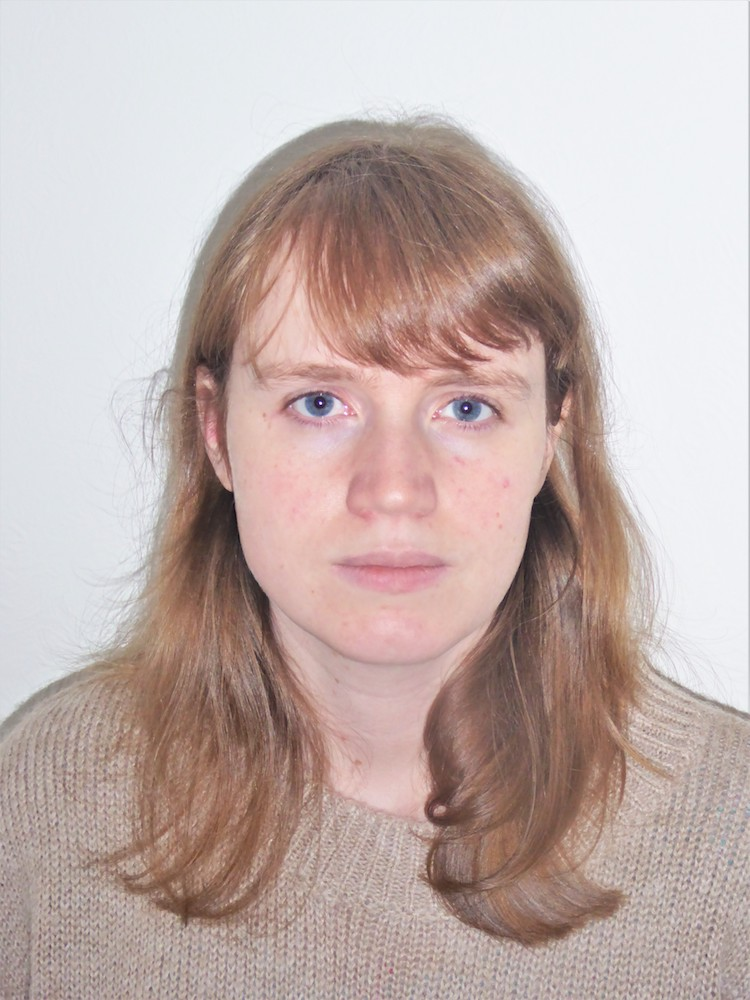
\includegraphics[width=0.2\textwidth]{1-introduction/img/natalie-lawton.jpg} & \textbf{Natalie Lawton - Management and Electrical Division}

\smallskip
\textit{Current Education}: MSc in Spacecraft Design.

\smallskip
\textit{Previous Education}: MEng in Aerospace Engineering. Previous experience in UAV avionic systems and emissions measurement techniques.

\smallskip
\textit{Responsibilities}: Acting as  Systems Engineer/Project Manager from the CDR until the end of the project. Previously was acting as deputy to these roles and in the electrical division. Ensures testing is planned and executed. Oversees manufacture, maintaining coordination between different teams and preventing project creep. Coordinating between different teams, project stakeholders, and documentation efforts. 
\bigskip
\\

 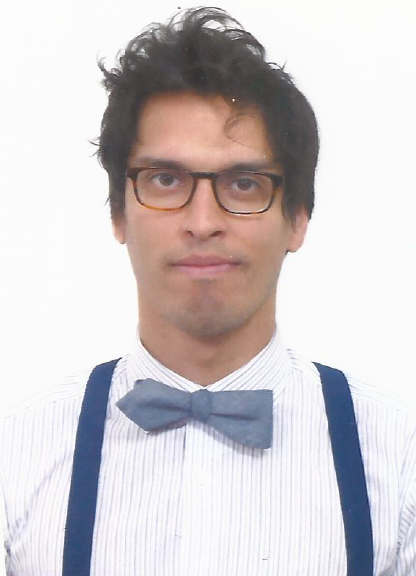
\includegraphics[width=0.2\textwidth]{1-introduction/img/georges-louis-joseph-labreche.jpg}  & \textbf{Georges L. J. Labrèche - Management Division}

\smallskip
\textit{Current Education}: MSc in Spacecraft Design.

\smallskip
\textit{Previous Education}: BSc in Software Engineering with experience in technical leadership and project management in software development.

\smallskip
\textit{Responsibilities}: Acting as Systems Engineer / Project Manager and managing overall implementation of the project until the Critical Design Review (CDR). Establishing and overseeing product development cycle. Coordinating between different teams, project stakeholders, and documentation efforts.                          
\bigskip
\\

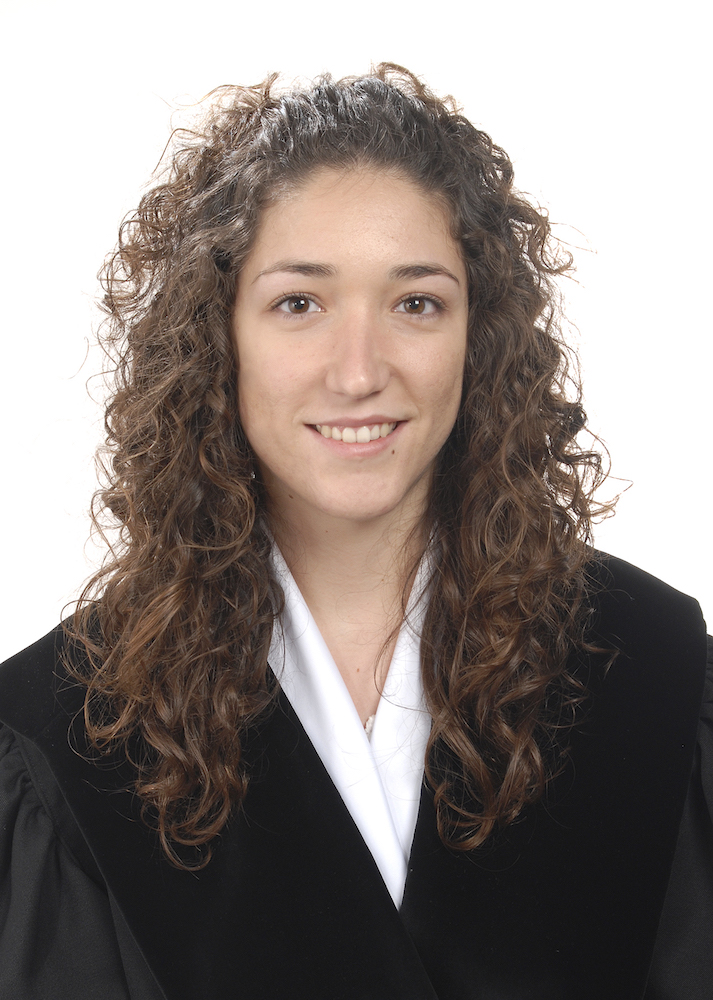
\includegraphics[width=0.2\textwidth]{1-introduction/img/agues-paszkowsky.jpg} & \textbf{Nuria Agües Paszkowsky - Scientific Division}

\smallskip
\textit{Current Education}: MSc in Earth Atmosphere and the Solar System.

\smallskip
\textit{Previous Education}: BSc in Aerospace Engineering.

\smallskip
\textit{Responsibilities}: Defining experiment parameters; data analysis; interpreting and documenting measurements; research on previous CAC experiments for comparative analysis purposes; contacting researchers or institutions working on similar projects; exploring potential partnership with researchers and institutions, evaluating the reliability of the proposed AAC sampling system; conducting measurements of collected samples; documenting and publishing findings. 
\bigskip
\\

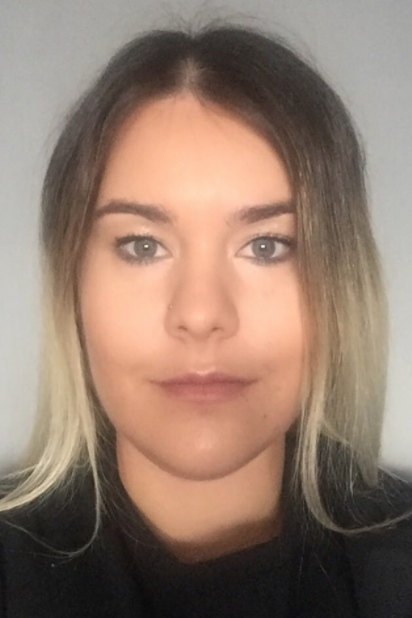
\includegraphics[width=0.2\textwidth]{1-introduction/img/kiki-blazaki.jpg} & \textbf{Kyriaki Blazaki - Scientific Division}

\smallskip
\textit{Current Education}: MSc in Earth Atmosphere and the Solar System.

\smallskip
\textit{Previous Education}: BSc in Physics.


\smallskip
\textit{Responsibilities}: Coordinating between the Scientific Division and the Project Manager; defining experiment parameters; data analysis; interpreting and documenting measurements; research on previous CAC experiments for comparative analysis purposes; evaluating the reliability of the proposed AAC sampling system; conducting measurements of collected samples; documenting and publishing findings. 
\bigskip
\\

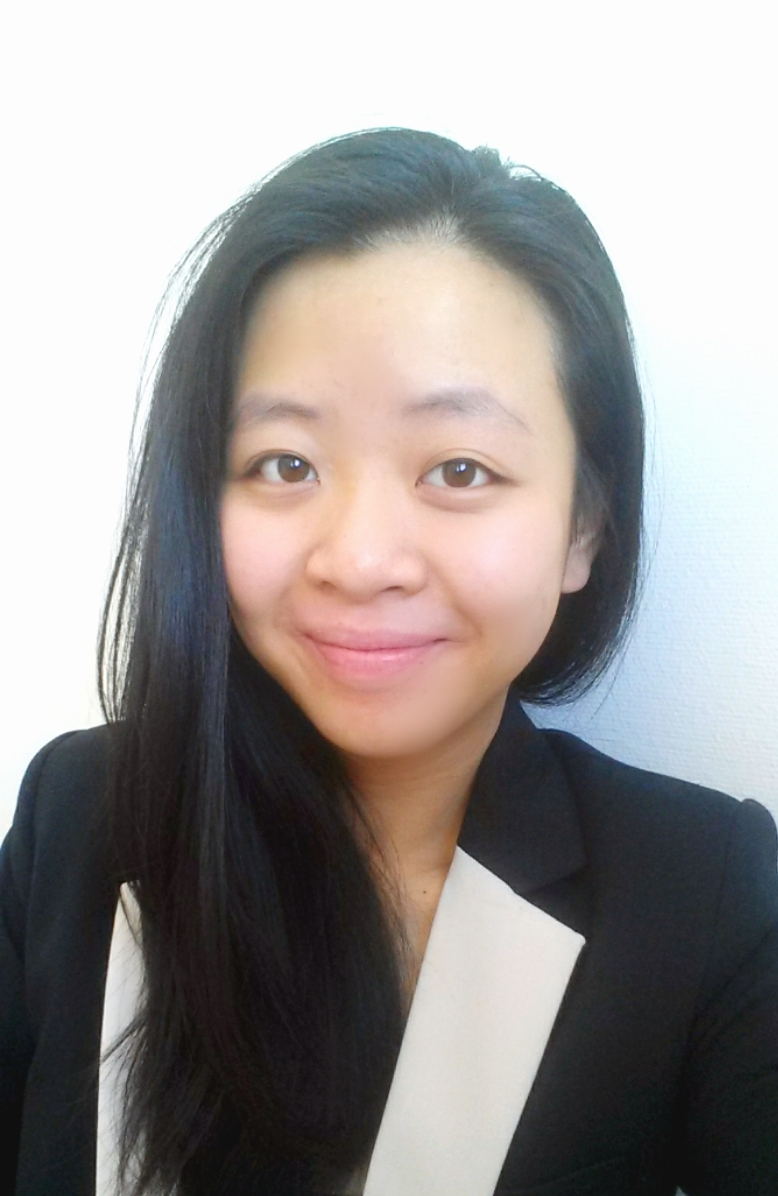
\includegraphics[width=0.2\textwidth]{1-introduction/img/emily-chen.jpeg} & \textbf{Emily Chen - Mechanical Division}

\smallskip
\textit{Current Education}: MSc in Space Engineering (5th Year).


\smallskip
\textit{Responsibilities}: Mechanical designing and assembly of CAC subsystem; analyzing the test results and changing the design as needed in collaboration with the team leader; integrating and assembling final design. 
\bigskip
\\

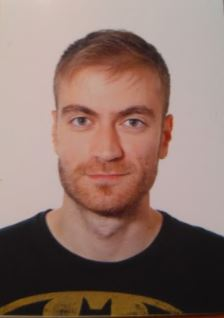
\includegraphics[width=0.2\textwidth]{1-introduction/img/jordi-coll-ortega.jpg} & \textbf{Jordi Coll Ortega - Mechanical Division}

\smallskip
\textit{Current Education}: MSc in Spacecraft Design.

\smallskip
\textit{Previous Education}: BASc in Aerospace Vehicle Engineering.

\smallskip
\textit{Responsibilities}: Designing or redesigning cost-effective mechanical devices using analysis and computer-aided design; developing and testing prototypes of designed devices; analyzing the test results and changing the design as needed in collaboration with the team lead; integrating and assembling final design.
\bigskip
\\


\includegraphics[width=0.2\textwidth]{1-introduction/img/gustav-dryssen.jpg} & \textbf{Gustav Dyrssen - Software Division}

\smallskip
\textit{Current Education}: MSc in Space Engineering (5th Year).

\smallskip
\textit{Responsibilities}: Leading quality assurance and testing efforts; Enforcing software testing best practices such as continuous integration testing and regression testing; reviewing requirements and specifications in order to foresee potential issues; provide input of functional requirements; advising on design; formalizing test cases; tracking defects and ensuring their resolution; facilitating code review sessions; supporting software implementation efforts.     
\bigskip
\\



\includegraphics[width=0.2\textwidth]{1-introduction/img/erik-fagerstrom.jpg} & \textbf{Erik Fagerström - Thermal Division}

\smallskip
\textit{Current Education}: MSc in Space Engineering (5th Year).


\smallskip
\textit{Responsibilities}: Coordinating between the Thermal Division and the Project Manager. Planning project thermal analysis and testing strategy. Thermal simulations of proposed designs and analyze results.
\bigskip
\\


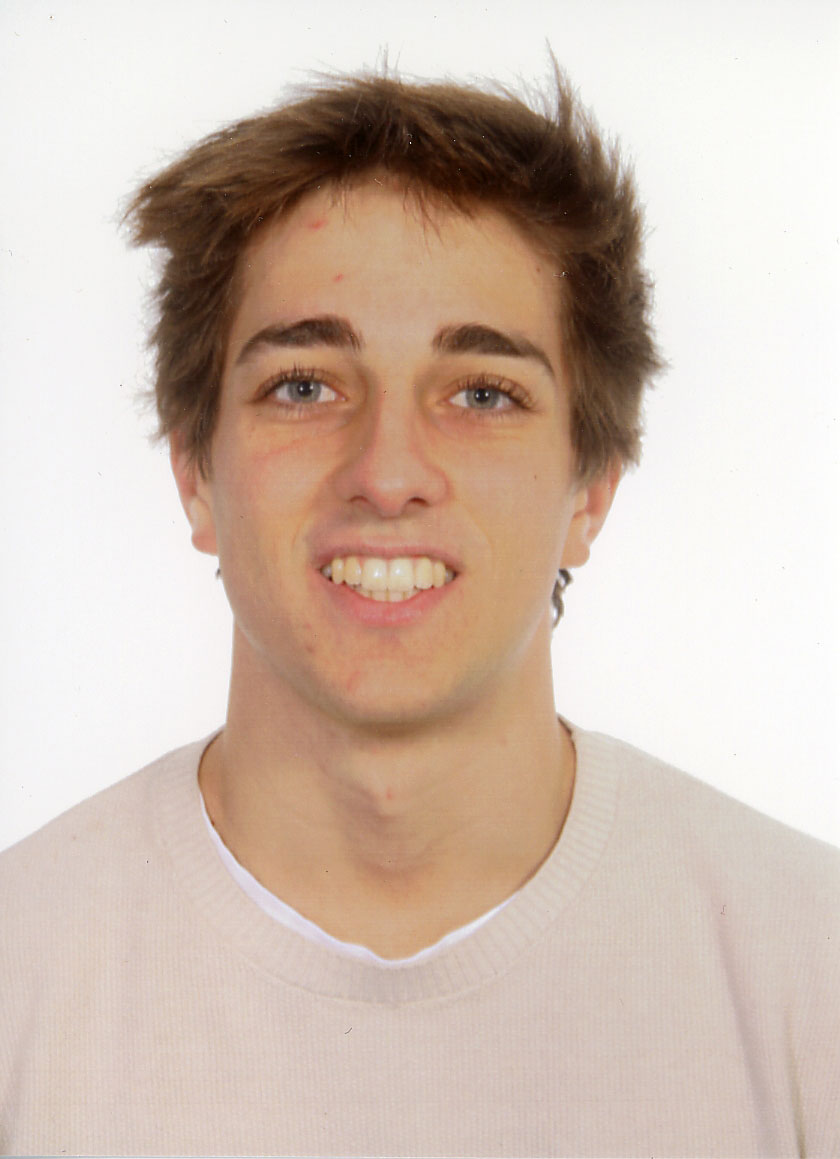
\includegraphics[width=0.2\textwidth]{1-introduction/img/pau-molas-roca.jpg} & \textbf{Pau Molas Roca - Mechanical Division}

\smallskip
\textit{Current Education}: MSc in Spacecraft Design.

\smallskip
\textit{Previous Education}: BSc in Aerospace Technology Engineering, Mechanical experience.

\smallskip
\textit{Responsibilities}: Coordinating between the Mechanical Division and the Project Manager; designing or redesigning cost-effective mechanical devices using analysis and computer-aided design; producing details of specifications and outline designs; overseeing the manufacturing process for the devices; identifying material and component suppliers; integrating and assembling final design.   \bigskip
\\


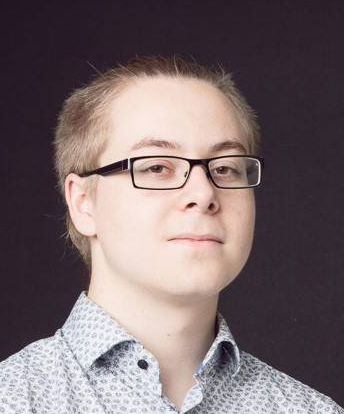
\includegraphics[width=0.2\textwidth]{1-introduction/img/emil-nordqvist.jpg} & \textbf{Emil Nordqvist - Electrical Division}

\smallskip
\textit{Current Education}: MSc in Space Engineering (5th Year).

\smallskip
\textit{Responsibilities}: Quality assurance of circuit design and implementation. Developing, testing, and evaluating theoretical designs.  \bigskip
\\

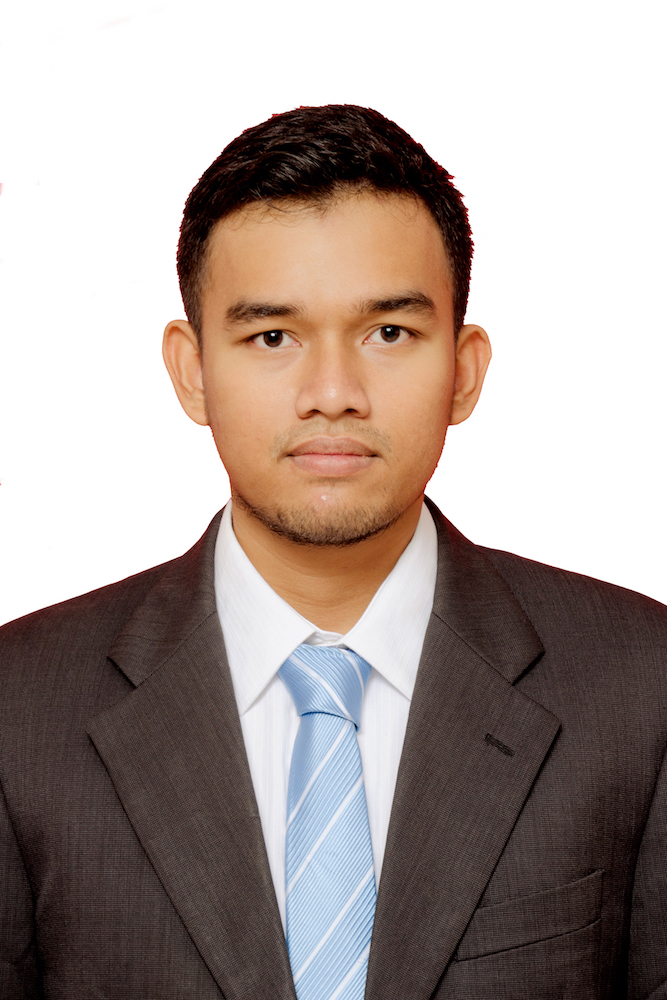
\includegraphics[width=0.2\textwidth]{1-introduction/img/muhammad-ansyar-rafi-putra.jpg} & \textbf{Muhammad Ansyar Rafi Putra - Software Division}

\smallskip
\textit{Current Education}: MSc in Spacecraft Design.

\smallskip
\textit{Previous Education}: BSc in Aerospace Engineering.


\smallskip 
\textit{Responsibilities}: Coordinating between the Software Division and the Project Manager; gathering software requirements; formalizing software specifications; drafting architecture design, detailed design; leading software implementation efforts.
\bigskip
\\

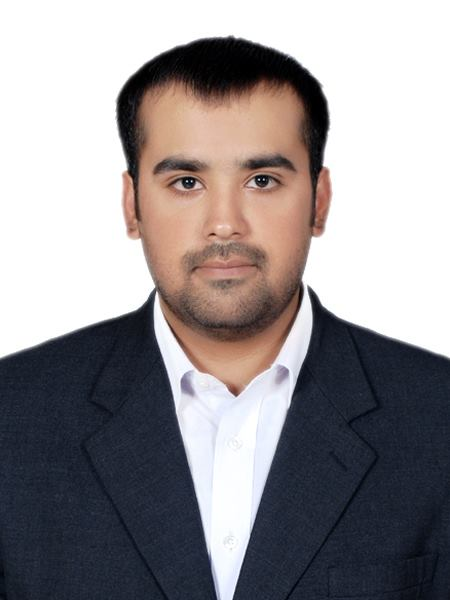
\includegraphics[width=0.2\textwidth]{1-introduction/img/hamad-saddiqi.jpg} & \textbf{Hamad Siddiqi - Electrical Division}


\smallskip
\textit{Current Education}: MSc Satellite Engineering.

\smallskip
\textit{Previous Education}: BSc in Electrical Engineering with experience in telecommunication industry and electronics.

\smallskip
\textit{Responsibilities}: Coordinating between the Electrical Division and the Project Manager; designing and implementing cost-effective circuitry using analysis and computer-aided design; producing details of specifications and outline designs; developing, testing, and evaluating theoretical designs; identifying material as well as component suppliers. 
\bigskip
\\


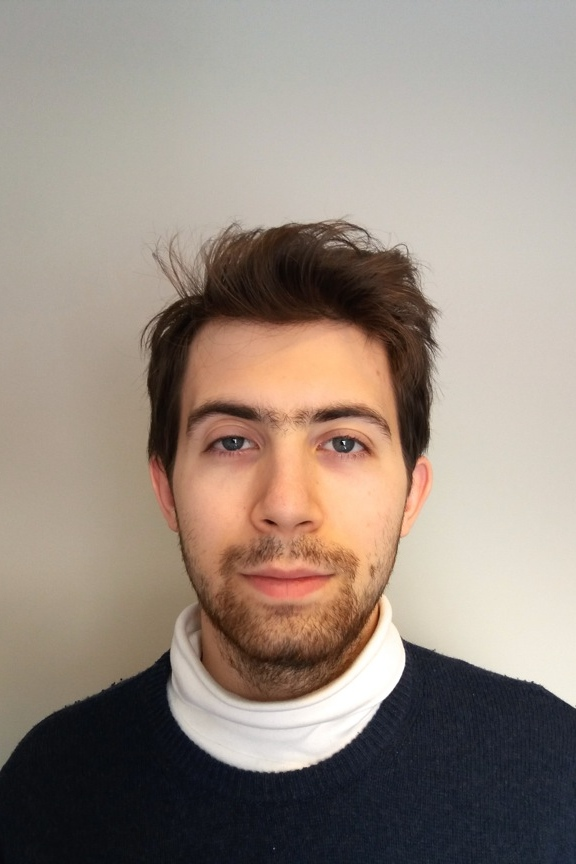
\includegraphics[width=0.2\textwidth]{1-introduction/img/ivan-zankov.jpg} & \textbf{Ivan Zankov - Thermal Division}

\smallskip
\textit{Current Education}: MSc in Spacecraft Design.

\smallskip
\textit{Previous Education}: BEng in Mechanical Engineering.

\smallskip
\textit{Responsibilities}: Thermal analysis of proposed designs and analysis result based recommendations.                                                         

\\
\label{tab:people}
\end{longtable}
\raggedbottom